\documentclass[a4paper]{article}

% here is a comment made from my phone
% here is anither comment fron my phone

\usepackage{pgfplots}
    \pgfplotsset{compat=1.17}
\usepackage{graphicx}
    \graphicspath{{./images/}}
\usepackage{amsmath}
\usepackage{amsthm}
\usepackage{caption}
\usepackage{subcaption}
\usepackage{booktabs}
\usepackage[style = apa]{biblatex}
    \addbibresource{references.bib}
\usepackage[breaklinks]{hyperref}
    \hypersetup{
        hidelinks,
        breaklinks=true
    }


\title{Problem Solving and Modelling Task}
\author{Alexander Arthur}

\hbadness=10000
\hfuzz=100pt

\theoremstyle{definition}
\newtheorem{assumption}{Assumption}
\newtheorem{observation}{Observation}

\begin{document}

\maketitle
\setcounter{tocdepth}{1}
\tableofcontents


\section{Introduction}
    The given task is to predict the date on which a population of bacteria will completely cover the surface of the water in a dam (Figure \ref{figDamOutline}). In order to do this, the area of the lake must first be calculated from the diagram provided. Once this area is known, the growth of the bacteria can then be projected and used to calculate the point at which the lake will be covered.

    \begin{figure}
        \centering
        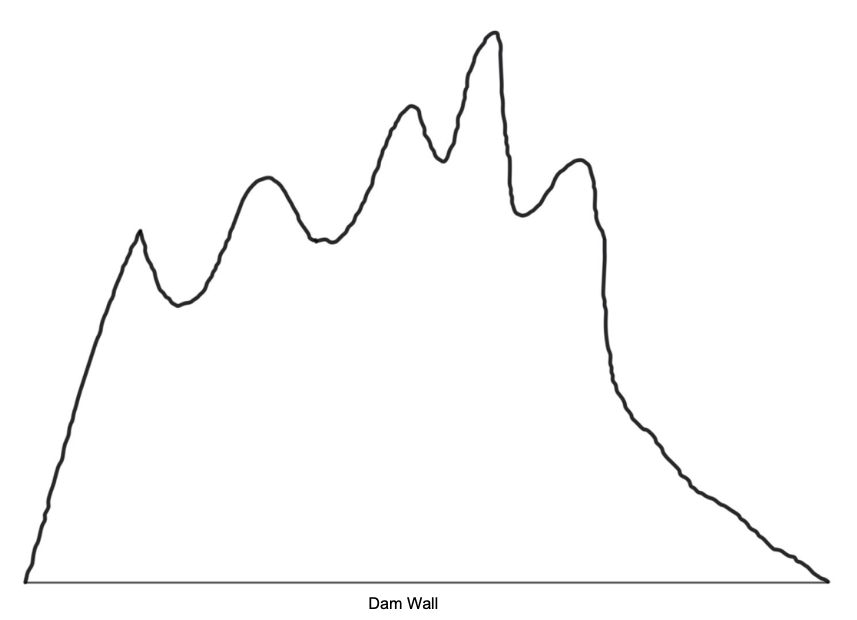
\includegraphics[width = 8cm]{damDiagram.png}
        \caption{Diagram of outline of dam}
        \label{figDamOutline}
    \end{figure}



\section{Assumptions and observations}

    \subsection{Observations}

        \begin{observation}
            When the diagram of the dam is oriented with the straight wall colinear with the $x$-axis, the rest of the outline passes the vertical line test, meaning that it can be modelled with a mathematical function.
        \end{observation}

        \begin{observation}
            The area covered by the bacteria increases each day, suggesting that it will eventually increase to be larger than that of the dam.
        \end{observation}
    
    \subsection{Assumptions}
    
        In order to simplify the problem, certain assumptions must be made either due to a lack of information provided or to bring the scope of the problem to a reasonable scale.

        \begin{assumption}
            If the water level of the dam were to change the water's surface area would also change, since it is unlikely the walls of the dam are perfectly vertical. Changing the surface area of the dam would in turn affect the point at which the bacteria would cover the entire lake, affecting the result of the investigation. Since no data is provided on the water level, it is reasonable to assume that it is static, and will not have any effect on the surface area of the lake.
        \end{assumption}

        \begin{assumption} \label{asmptnBacteriaGrowth}
            In a similar vein, there are many factors which can influence the growth rate of a population of bacteria, including access to a food source, temperature and competition for space. Similarly to the dam's water level, no data is provided around this, meaning that it must be assumed that the none of these factors will affect the bacteria as the population grows.
        \end{assumption}
        
\section{Translation of mathematical concepts}
    
    As per the requirements of the task, a mathematical approach must be used to calculate the area of the dam. To satisfy this requirement, the definite integral of a piecewise function will be used to calculate the area of the dam.

    In statistical modelling, a model can be overfitted to a dataset such that it is highly accurate within the domain of the data, but is wildly inaccurate outside this domain, meaning that it cannot be used to predict values outside the domain of the data and therefore is not useful. However, in this task, for any given segment of the piecewise function the only domain which is applicable is that of that segment, meaning that the concept of the function being over-fitted does not apply. In addition, the Weierstrass approximation theorem states that for any continuous function $f$ over the real interval $[a, b]$ and any $\epsilon > 0$ there exists a polynomial $p$ such that $|f(x) - p(x)| < \epsilon$, where $a \leq x \leq b$.
 
    This means that since the only key metric used to select a function is its accuracy within the specified domain, regression was used to select a function within each defined section, and the regression models used were strictly polynomial; the degree of the polynomial was simply increased until the function fit the data to a sufficient degree of accuracy ($R^2 > 0.97$).

    To generate the points to be used for these regressions, a Python script was written to list the coordinates of the topmost black pixel in each column of pixels. This generated a list of 1262 pixel coordinates, which were scaled to the dimensions of the dam such that one unit on the $x$ and $y$ axes were each equal to 1 meter and subsequently used to generate regression models (Figure \ref{figRawData}).

    \begin{figure} % Raw data
        \centering
        \begin{tikzpicture}
            \begin{axis}[
                    title = {\textbf{Raw data points}},
                    xmajorgrids = true,
                    ymajorgrids = true
                ]
                \addplot[only marks, mark = x]table[x=x, y=y]{data/data.txt};
            \end{axis}
        \end{tikzpicture}
        \caption{Raw data from Python script}
        \label{figRawData}
    \end{figure}

    In an ideal scenario, a single function could be used to model the entire length of the dam's outline. However, due to the computational limits of the available software a polynomial regression of sufficiently high degree is not possible. This means that the data was instead divided into several sections (Figure \ref{figSectionedData}), each of which were then  used to run a polynomial regression. Since these sections were selected to have more simple shapes than the entire dataset, polynomials of much lower degree ($< 6$) were sufficient to replicate their shape to a sufficient degree of accuracy.

    \begin{figure} % Sectioned data
        \centering
        \begin{tikzpicture}
            \begin{axis}[
                    title = {\textbf{Sectioned data}},
                    xmajorgrids = true,
                    ymajorgrids = true
                ]
                \addplot[only marks, mark = x, color = red]table[x=x1, y=y1]{data/section1.txt};
                \addplot[only marks, mark = x, color = blue]table[x=x2, y=y2]{data/section2.txt};
                \addplot[only marks, mark = x, color = red]table[x=x3, y=y3]{data/section3.txt};
                \addplot[only marks, mark = x, color = blue]table[x=x4, y=y4]{data/section4.txt};
                \addplot[only marks, mark = x, color = red]table[x=x5, y=y5]{data/section5.txt};
                \addplot[only marks, mark = x, color = blue]table[x=x6, y=y6]{data/section6.txt};
                \addplot[only marks, mark = x, color = red]table[x=x7, y=y7]{data/section7.txt};
                \addplot[only marks, mark = x, color = blue]table[x=x8, y=y8]{data/section8.txt};
            \end{axis}
        \end{tikzpicture}
        \caption{Data shown in coloured sections}
        \label{figSectionedData}
    \end{figure}

    \subsection{Calculation of area}

        Let us define a variable $b$ for the boundaries between the sections, such that $b_0 = 0$, $b_1 = 4.3$ \ldots $b_8 = 30$. Let us also  define the piecewise function $f$ as follows (Figure \ref{figDamFunction}):

        \begin{equation} % Piecewise function
            f(x) = \begin{cases}
                f_1(x) & b_0 \leq x < b_1 \\
                f_2(x) & b_1 \leq x < b_2 \\
                \vdots & \vdots \\
                f_7(x) & b_6 \leq x < b_7 \\
                f_8(x) & b_7 \leq x \leq b_8
            \end{cases}
            \label{eqnPiecewiseFunction}
        \end{equation}

        \begin{figure} % Dam function from desmos
            \centering
            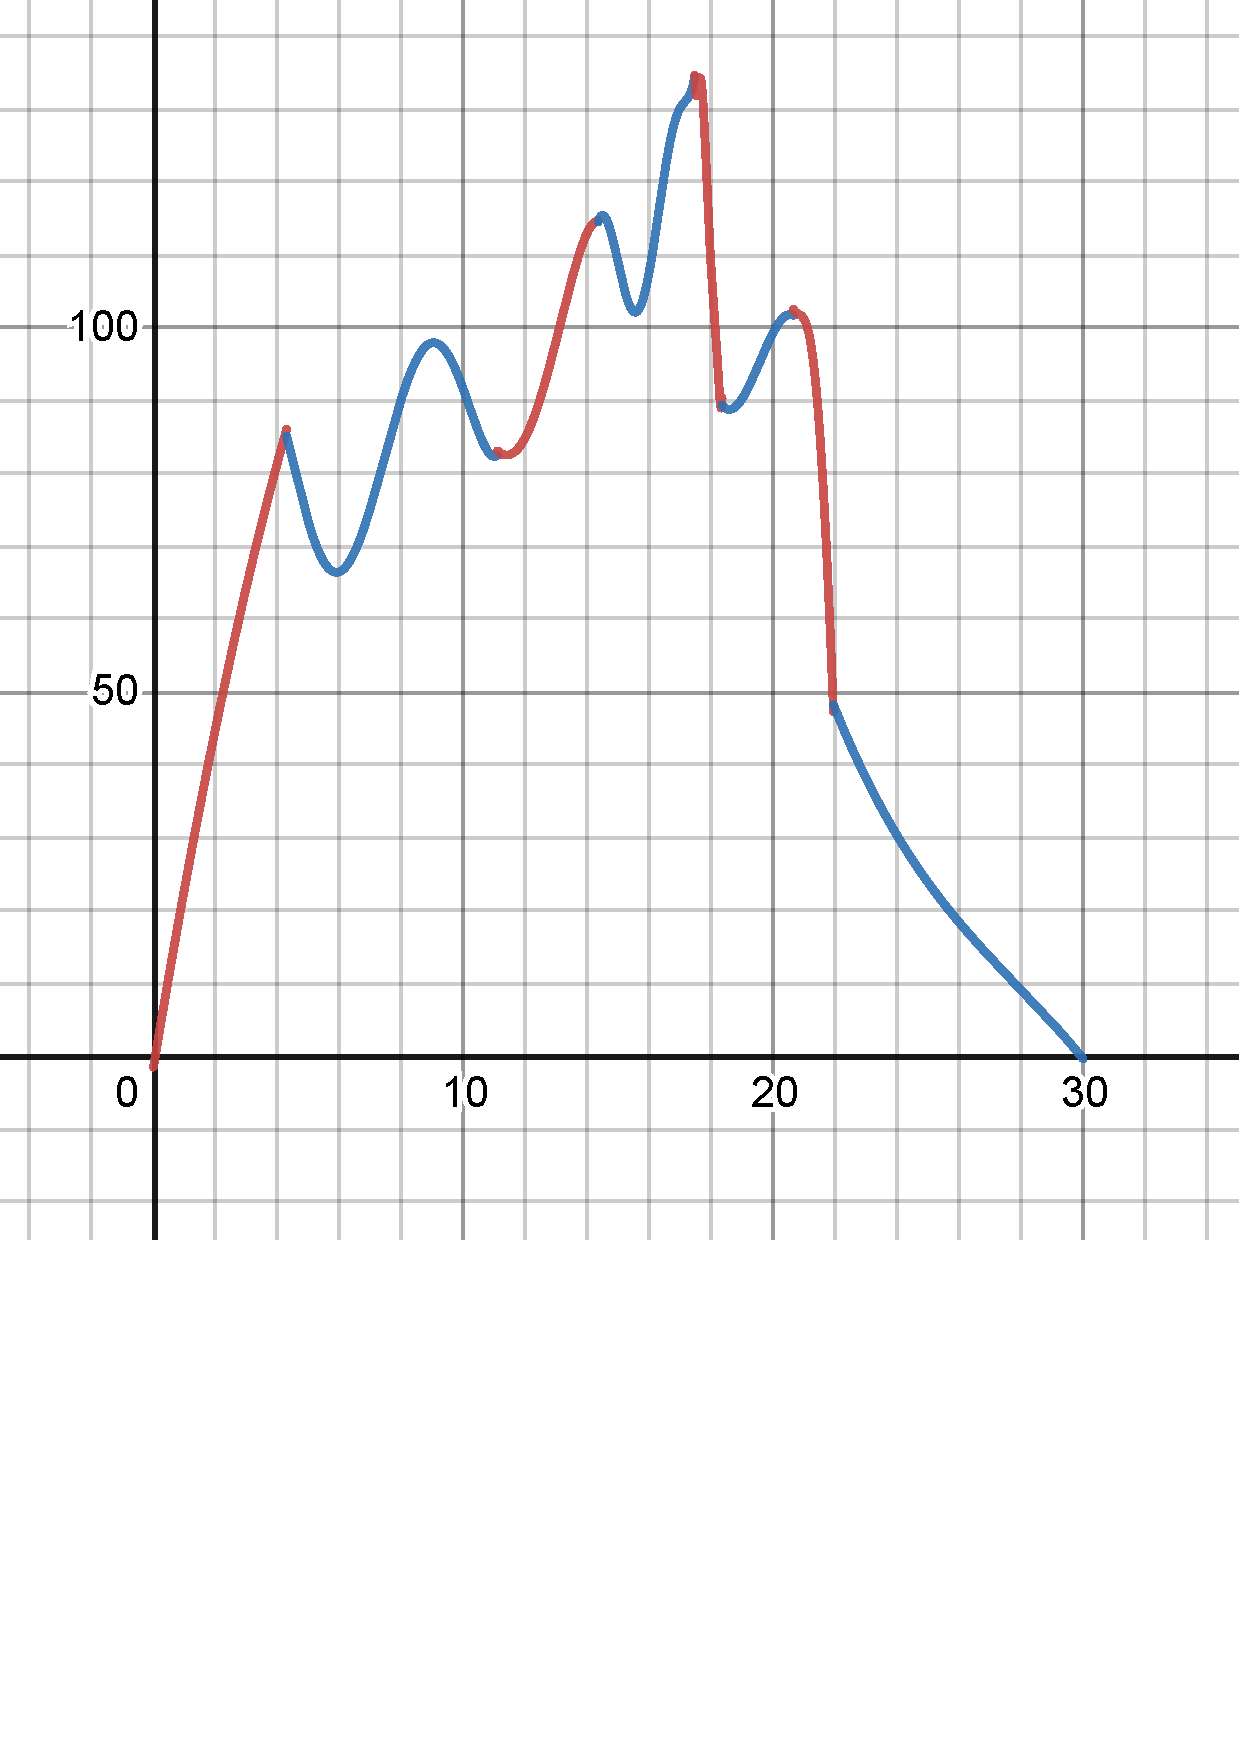
\includegraphics[width = 8cm]{damFunction.pdf}
            \caption{Piecewise function modelling outline of dam}
            \label{figDamFunction}
        \end{figure}

        The values of $b_n$ were selected to create sections of data that were simple to create regression models for and are as follows:

        \begin{align*} % values of b_n
            b_0 &= 0 \\
            b_1 &= 4.3 \\
            b_2 &= 11.1 \\
            b_3 &= 14.4 \\
            b_4 &= 17.5 \\
            b_5 &= 18.4 \\
            b_6 &= 20.7 \\
            b_7 &= 22.0 \\
            b_8 &= 30
        \end{align*}

        The subfunctions $f_1 \cdots f_8$ were found using polynomial regression models and are defined as follows:

        \begin{align*} % Subfunctions of f
            f_1(x) &= -1.2364x^2 + 25.667x - 1.4657 \\
            f_2(x) &= 0.0922x^5 - 3.4033x^4 + 47.748x^3 - 315.07x^2 + 968.69x - 1022.9 \\
            f_3(x) &= -0.4898x^4 + 22.736x^3 - 388.82x^2 + 2903.4x - 7897 \\
            f_4(x) &= 1.1895x^6 - 110.38x^5 + 4255.2x^4 - 8.7230\cdot 10^04x^3 + 1.0027\cdot 10^6x^2 \\ &- 6.1276\cdot 10^6x + 1.5551\cdot 10^7 \\
            f_5(x) &= 6046.8x^6 - 6.5135 \cdot 10^5x^5 + 2.9233 \cdot 10^7x^4 - 6.9967 \cdot 10^8x^3 \\ &+ 9.4192 \cdot 10^9x^2 - 6.7624 \cdot 10^{10}x + 2.0228 \cdot 10^{11} \\
            f_6(x) &= -3.4000x^3 + 199.63x^2 - 3897.0x + 25388 \\
            f_7(x) &= 253.31x^5 - 26978x^4 + 1.1491 \cdot 10^6x^3 - 2.4471 \cdot 10^7x^2 + 2.6052 \cdot 10^8x \\ &- 1.1093 \cdot 10^9 \\
            f_8(x) &= -0.0556x^3 + 4.6621x^2 - 134.73x + 1347.2
        \end{align*}

        Using the subfunctions of $f$, the area $A$ inside the lake can be calculated using the sums of the definite integrals of each function $f_n(x)$ within its applicable domain $b_{n-1} \leq x < b_n$, otherwise expressed as:

        \begin{equation}\label{eqnAreaOfLakeFromFuncs}
           A = \sum_{n=1}^8 \int_{b_{n-1}}^{b_n} f_n(x)\,dx
        \end{equation}

        This process will now be demonstrated for $n = 1$:
        \begin{align*} % Manual calcs
            A_1 =& \int_{b_0}^{b_1} f_1(x)dx \\
            =& \int_{0}^{4.3} \left(-1.2364x^2 + 25.667x - 1.4657\right)dx \\
            =& \left[-0.41213x^3 + 12.8335x^2 - 1.4657x\right]_0^{4.3} \\
            =& (-0.41213 \cdot 4.3^3 + 12.8335 \cdot 4.3^2 - 1.4657 \cdot 4.3) \\ &- (-0.41213 \cdot 0^3 + 12.8335 \cdot 0^2 - 1.4657 \cdot 0) \\
            =& 198.2217
        \end{align*}

        Using Equation \ref{eqnAreaOfLakeFromFuncs}, the area of the lake is 2027.9283m$^2$.


    \subsection{Projection of bacteria growth}
    
        \cite{bacteriaGrowth} states that a population of bacteria will grow exponentially when under the conditions assumed in Assumption \ref{asmptnBacteriaGrowth}. This means that the growth of the population can be modelled using an exponential function of the form 
        \begin{equation}
            f(x)=ae^{bx}
        \end{equation}

        Using an exponential regression model, the bacterial growth was found to fit the function $f(x) = 1.66918e^{0.284009x}$ with an $R^2$ value of 0.9999 (Figure \ref{figBacteriaGrowth})
        \begin{figure}
            \centering
            \begin{tikzpicture}
                \begin{axis}[
                        title = {\textbf{Raw data points}},
                        xmajorgrids = true,
                        ymajorgrids = true,
                        legend pos = north west
                    ]
                    \addplot[only marks]table[x=x, y=y]{data/bacteriaData.txt};\addlegendentry{Data point}
                    \addplot[mark = none, domain = 0:20, smooth]{1.669188*e^(0.284009*x)};\addlegendentry{Regression model}
                \end{axis}
            \end{tikzpicture}
            \caption{Raw data and regression model of bacteria population}
            \label{figBacteriaGrowth}
        \end{figure}

        Using this regression model, the point at which the area covered by the bacteria can be found as follows:
        
        \begin{align*}
            2027.9283 &= 1.66918e^{0.284009x} \\
            \frac{2027.9283}{1.66918} &= e^{0.284009x} \\
            \ln 1214.92487329 &= 0.284009x \\
            x &= \frac{\ln 1214.92487329}{0.284009} \\
            x &= 25.00779032
        \end{align*} 

        This means that the dam will be entirely covered by bacteria on the 25\textsuperscript{th} of January.

\section{Evaluation}
    
    \subsection{Justification of mathematical procedures}

    \subsection{Reasonableness}
        The model 

    \subsection{Evaluation of model and result}

        \subsubsection{Strengths}
            The model had a very close fit with the data in each section ($R^2 > 0.97$), and was also very visually similar to the plot of the raw data (Figure \ref{figCompareDataAndFunction}). This indicates that the shape whose area was calculated matched that of the physical dam closely, and since the process of integration bears no inherent inaccuracies it is likely that the area calculated is highly accurate.

            Similarly, the model for the size of the bacteria population also had a very high $R^2$ value of 0.9999, indicating that it is also a very close fit for the data collected. An exponential function is also theoretically the correct type of function to model the size of a population of bacteria, since each generation the population multiplies by a certain amount when ignoring outside factors as per Assumption \ref{asmptnBacteriaGrowth}.

            Another strength of the model is the extent to which it makes use of computational resources to increase its accuracy. Using a Python script to generate the set of points used for regression greatly increases the number of points available without introducing any inaccuracies due to human error. This in turn makes the regression models generated more accurate due to this elimination of human error. 

            \begin{figure}
                \centering
                \begin{subfigure}[b]{0.4\textwidth}
                    \hfuzz=30pt
                    \centering
                    \begin{tikzpicture}
                        \begin{axis}[
                                scale only axis,
                                width = \textwidth,
                                xmajorgrids = true,
                                ymajorgrids = true
                            ]
                            \addplot[only marks, mark = x]table[x=x, y=y]{data/data.txt};
                        \end{axis}
                    \end{tikzpicture}
                    \caption{Raw data}
                \end{subfigure}
                \hfill
                \begin{subfigure}[b]{0.4\textwidth}
                    \hfuzz=30pt
                    \centering
                    \frame{
                        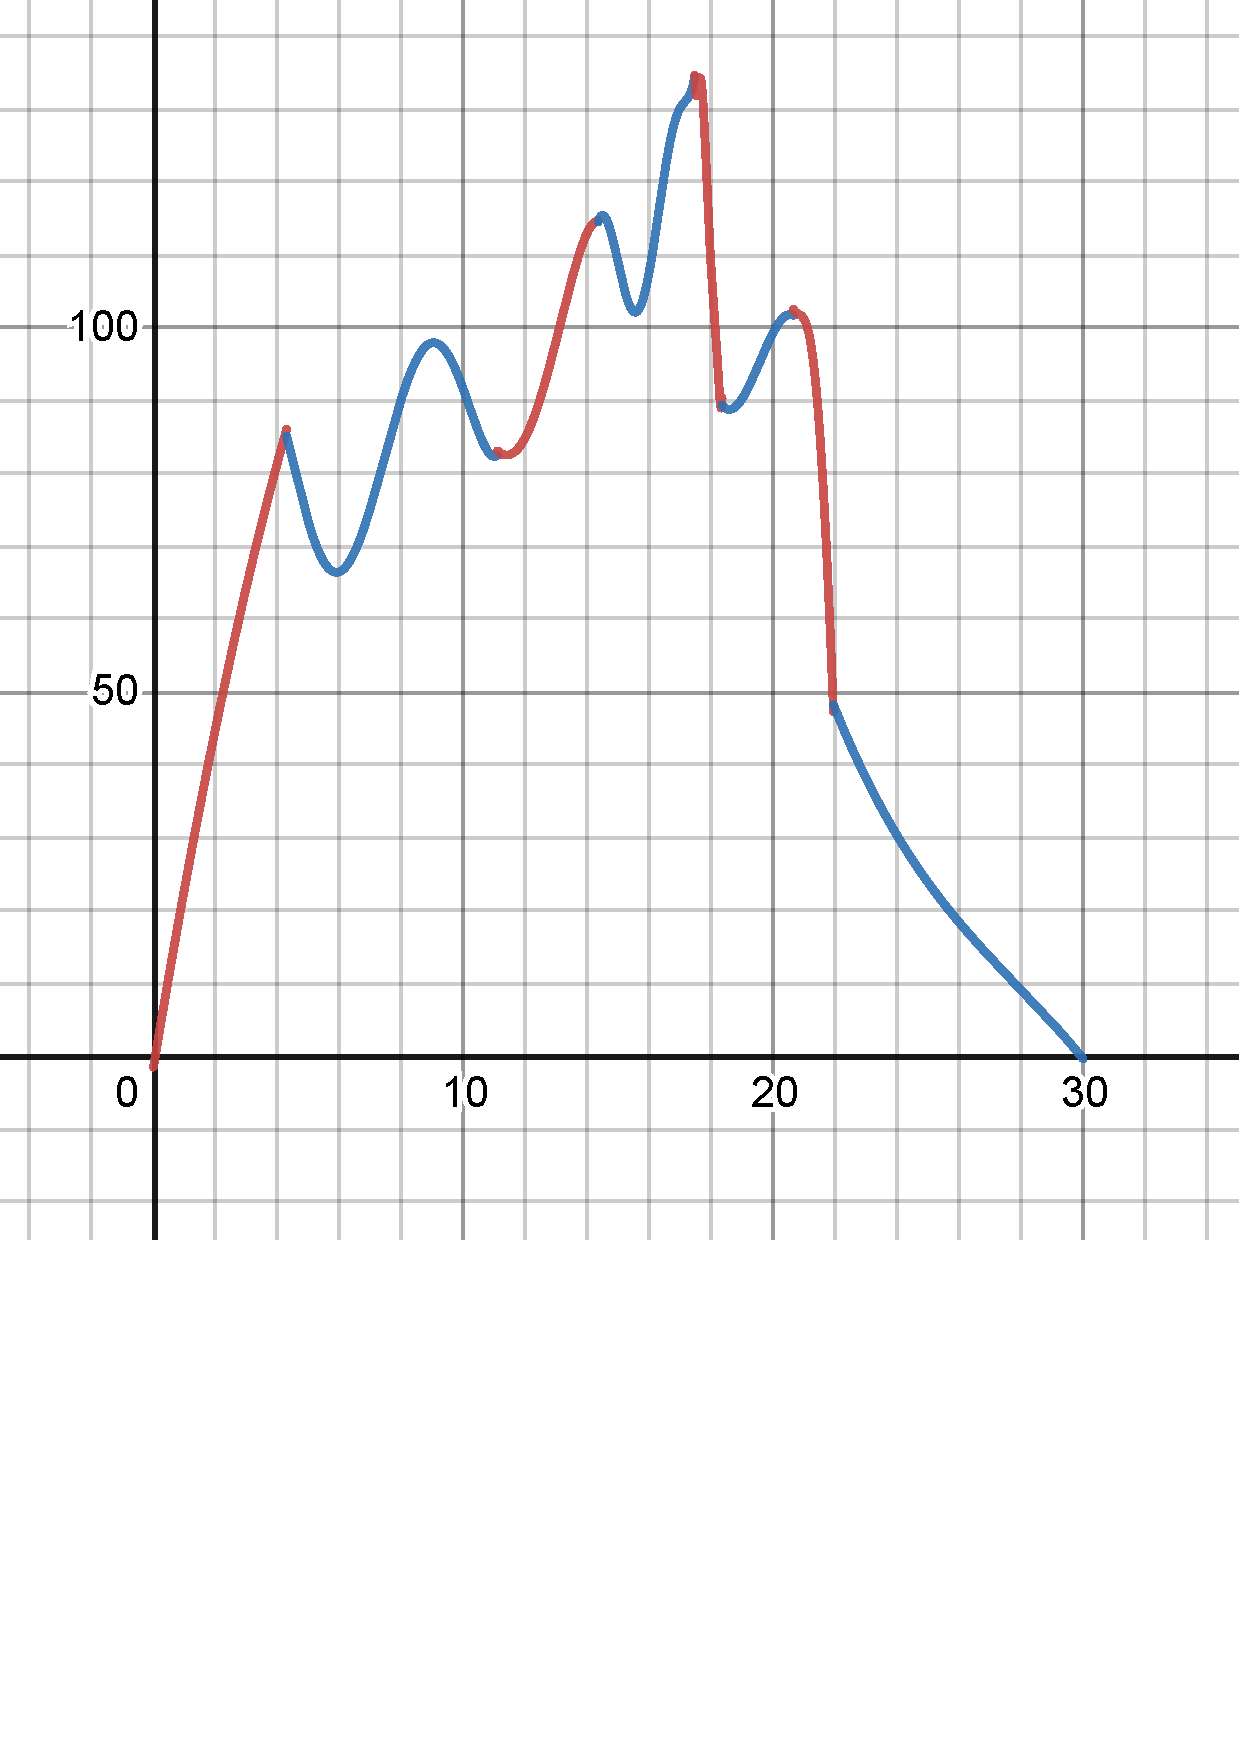
\includegraphics[width = \textwidth]{damFunction.pdf}
                    }
                    \caption{Piecewise function}
                \end{subfigure}
                \caption{Comparison of raw data and piecewise function}
                \label{figCompareDataAndFunction}
            \end{figure}


        \subsubsection{Limitations}

\section{Conclusion}



\printbibliography

\end{document}
